\documentclass{beamer}
\usetheme{Warsaw}

\newcommand{\page}{\textbf{p} }
\newcommand{\query}{\textbf{q} }
\newcommand{\keyword}{\textbf{w} }
\newcommand{\str}{\textbf{s} }
\newcommand{\cheap}{\textbf{candidate heap} }
\newcommand{\kheap}{\textbf{keyword heap} }
\newcommand{\topk}{\textbf{k} }
%\newcommand{\k}{\textbf{k} }

\begin{document}

\title{Estimating the ImpressionRank of Web Pages}
\author{FAN Kai \\ fankai@net.pku.edu.cn}
\institute{Computer Networks and Distritued Systems Laboratory\\Peking University}
\date{May 15, 2009}

\begin{frame}
    \titlepage
\end{frame}

\section{Introduction}
    \subsection{Problem}

    \begin{frame}{ImpressionRank}
        \begin{itemize}
        \item A measure of \textbf{exposure} of a web page/site in a search engine
        \item Number of times users viewed the page while browsing search results
        \item Page \page has an impression on a query(keyword) \query:
            \begin{itemize}
            \item the search engine return \page as a result for \query
            \item the user looked at the result(click is not necessary)
            \item \textbf{the top n ranking results}
            \end{itemize}
        \end{itemize}
    \end{frame}

    \begin{frame}{Motivation}
        \begin{itemize}
        \item  Popularity rating of pages and sites
            \begin{itemize}
            \item assume visibility is corelated with traffic
            \item Nielson, comScore and Alexa
            \end{itemize}
        \item  Site analytics
            \begin{itemize}
            \item impressions vs. clicks
            \end{itemize}
        \item  Market research
            \begin{itemize}
            \item different sites
            \item different queries
            \item different search engines
            \end{itemize}
        \item  Search engine evaluation
            \begin{itemize}
            \item impressions of spams, hate sites, porn and virus infected pages
            \end{itemize}
        \end{itemize}
    \end{frame}

    \begin{frame}{Contribution}
        \begin{itemize}
        \item First \textbf{external} algorithm for popular keyword extraction
            \begin{itemize}
            \item the search engine
            \item the query suggestion service
            \item the web
            \end{itemize}
        \item Moderst Resource
            \begin{itemize}
            \item search engine requests(hundreds)
            \item suggestion service requests(tens of thousands)
            \item fetch web pages(hundreds)
            \end{itemize}
        \end{itemize}
    \end{frame}

    \subsection{Methodology}

    \begin{frame}{Challenges}
        \begin{itemize}
        \item find queries for which the search engine would return a certain page
        \item find how many impressions these queries generate
        \item limits on the rate of requests posed by search engine
        \end{itemize}
    \end{frame}

    \begin{frame}{ImpressionRank Calculation}
        \begin{itemize}
        \item Notions
            \begin{itemize}
            \item \textbf{impression(p,w)} impression contribution of keyword \keyword to page \page
            \item \textbf{incident(p,w)} whether the search engine return \page for \keyword
            \item \textbf{freq(w)} number of \keyword in the query log
            \item \textbf{N(p)} neighbors of page \page, or all keywords incident to \page
            \end{itemize}
        \item Formula
            \begin{itemize}
            \item $ impression(p, w) = incident(p, w) \cdot freq(w) $
            \item $ irank(p) = \sum_{w}impression(p,w) = \sum_{w\in neighbor(p)}freq(w) $
            \item $ irank(website) = \sum_{p\in website}irank(p) $
            \end{itemize}
        \end{itemize}
    \end{frame}

    \begin{frame}{Popular Keyword Extraction}
        \begin{itemize}
        \item Power law distribution of query frequencies
            \begin{itemize}
            \item 73\% impressions of www.cnn.com come from "cnn", "election results", "news"
            \item assume power law holds for a specific document
            \end{itemize}
        \item Varient of classical keyword extraction problem
            \begin{itemize}
            \item find impressions on top queries
            \end{itemize}
        \item Algorithm
            \begin{itemize}
            \item use the frequencies of the top k keywords to infer the exponent of power law
            \item sum up the total frequency to estimate the ImpressionRank
            \end{itemize}
        \end{itemize}
    \end{frame}

    \begin{frame}{Remaining Problems}
        \begin{itemize}
        \item Keyword Frequency Estimation
            \begin{description}
            \item [Input] A keyword \keyword
            \item [Output] The frequency of \keyword in search engine log
            \end{description}
        \item Popular Keyword Extraction
            \begin{description}
            \item [Input] A document \page and an integer \textbf{k}
            \item [Output] The \textbf{k} keywords on which \page has the most impressions
            \end{description}
        \end{itemize}
    \end{frame}

\section{Frequency Estimation}
    \subsection{Introduction}
    \begin{frame}{Suggestion Services}
        \begin{itemize}
        \item Given a string \str, suggesting service returns the most popular queries which starts with \str.
        \item \em{VLDB 2008, Mining Search Engine Query Logs via Suggestion Sampling}
        \end{itemize}
        \begin{figure}
        \includegraphics[width=100mm]{trie}
        \end{figure}
    \end{frame}

    \begin{frame}{Frequency vs. Volume}
        \begin{itemize}
        \item Notions
            \begin{description}
            \item [freq(q)] frequency of a query \query \\
                \em{number of instances \query in the query log}
            \item [vol(s)] volume of a string \str  \\
                \em{number of distinct queries in the log of whom \str is a prefix}
            \item [pre(q)] shortest exposing prefix of a query \query  \\
                \em{shortest prefix \str of \query for which the suggestion service return \query as one of the suggestions for \str}
            \end{description}
        \item Correlation between \textbf{freq(q)} and \textbf{vol(pre(q))}
            \begin{itemize}
            \item both have power law distributions
            \item "order-corelated"
            \item measure \textbf{freq(q)} using \textbf{vol(pre(q))}
            \end{itemize}
        \item How to find \textbf{pre(q)}?
        \end{itemize}
    \end{frame}

    \subsection{Volume Estimation}
    \begin{frame}{Naive Volume Calculator}
        \begin{itemize}
        \item Assume suggestion service return M results at most each time.
        \item If we send a string \str to suggestion service and the service return $ k(<M) $ results, we could infer $ vol(s) = k $ .
        \item If suggestion service return$ k(\ge M) $ results, recursively computes the volumes of the children of \str and sum them up.
        \end{itemize}
    \end{frame}

    \begin{frame}{Real Volume Estimator}
        \begin{itemize}
        \item Naive estimator
            \begin{equation*}
            VolEst_{naive}(s)=\left\{
                \begin{array}{rl}
                    |results(s)|, & \text{if } |results(s) < M \\
                    a, & \text{if } k \ge M
                \end{array} \right.
            \end{equation*}
        \item Sample-based estimator \\
            given $ T' \text{is a random sample of } T $
            \begin{equation*}
            VolEst_{sample}(s)=\left\{
                \begin{array}{rl}
                    vol(s, T') \cdot \frac{|T|}{|T'|}, & \text{if } |vol(s, T') \ge b \\
                    0, & otherwise
                \end{array} \right.
            \end{equation*}
        \item Score-based estimator
        \end{itemize}

        \begin{theorem}
        $ VolEst(s) = VolEst_{naive}(s) + VolEst_{sample}(s) + VolEst_{score}(s) $
        \end{theorem}
    \end{frame}


\section{Popular Keyword Extraction}

    \subsection{Overview}
    \begin{frame} {Overview}
        \begin{itemize}
        \item Impossible to test all keywords.
        \item Apply \em{best-first} search 
            \begin{itemize}
            \item track down the most promising candidates
            \item evaluate them
            \item report the top keywords found
            \end{itemize}
        \item \em{Cache} everything.
        \item Set requests budget.
        \end{itemize}
    \end{frame}

    \begin{frame}{Notions}
        \begin{itemize}
        \item \cheap : frontier of the search space
        \item \kheap : highest frequent keywords incident to document
        \item \textbf{seed text} : all related text to a web page
        \item \textbf{term pool} : all terms from \textbf{seed text}
        \item \textbf{candidate keywords} : all ordered finite-length sequences of terms from \textbf{term pool} 
        \end{itemize}
        \alert{search space} : a TRIE whose alphabet is all the terms
    \end{frame}

    \subsection{Main Flow}
    \begin{frame}{Main Flow}
        \begin{enumerate}
        \item crawl seed text, add all terms to \textbf{term pool} 
        \item \textbf{score} all terms and  insert them to \cheap
        \item loop while budget not reached
            \begin{enumerate}
            \item pop \keyword from \cheap and send to suggestion service
            \item $ S = \keyword \cup result(w) $
            \item for all $ u \in S $, if u is \textbf{incident} to page \page
                \begin{enumerate}
                \item \textbf{estimate} freq(u) and add to \kheap
                \item expand seed text with u and all pages incident to u 
                \item regenerate all terms, \textbf{recore}, and refresh \cheap
                \end{enumerate}
            \end{enumerate}
            \item expand \keyword
        \end{enumerate}
    \end{frame}

    \subsection{Subroutines}
    \begin{frame}{Test Incidence}
        \begin{itemize}
        \item Send keyword \keyword to search engine and check whether page \page is one of the top k results.
        \item Send query "inurl:url(p) w" to the search engine, if no results returned, then neither \keyword nor any of its descendants are incident to \page .
        \end{itemize}
    \end{frame}

    \begin{frame}{Whether To Expand A Candidate}
        \begin{itemize}
        \item diversity: if \keyword or any suggestions for \keyword already in \kheap, no need to expand
        \item if none of the descendants of \keyword has positive frequency, prune
        \item if none of the descendants of \keyword is incident to \page, prune
        \item if estimated frequency of the top descendant can not make top k in \kheap, prune
        \item otherwise, expand \keyword
        \end{itemize}
    \end{frame}

    \begin{frame}{Candidate Scoring}
        \begin{itemize}
        \item efficiency is important
        \item $ score(w) = score_{freq}(w)^a + score_{tf}(w)^b + score_{idf}(w)^c $
        \item estimate frequency score for w and all its descendants
            \begin{itemize}
            \item under budget
            \item estimate frequency for keywords r which has most descendants
                \begin{itemize}
                \item if vol(r) is 0 or 1, then all its descendants has no frequency
                \item if r is choosed, then its ancestors is also choosed
                \end{itemize}
            \item for keyword u which is not selected
                \begin{itemize}
                \item if r=pre(u) is selected, estimate its score by vol(pre(u))
                \item if r=pre(u) is not selected, find its lower-most ancestor r which has been selected, F is the sum of the frequencies of r's descendants not in suggestions,  $ score_{freq}(u) = \frac{F}{vol(r)-N}  $
                \end{itemize}
            \end{itemize}
        \end{itemize}
    \end{frame}

\section{Experiments \& Conclusion}
    \begin{frame}[plain]{Query Popularity}
        \begin{figure}
        \includegraphics[width=100mm]{powerlaw}
        \end{figure}
    \end{frame}

    \begin{frame}[plain]{Recall}
        \begin{figure}
        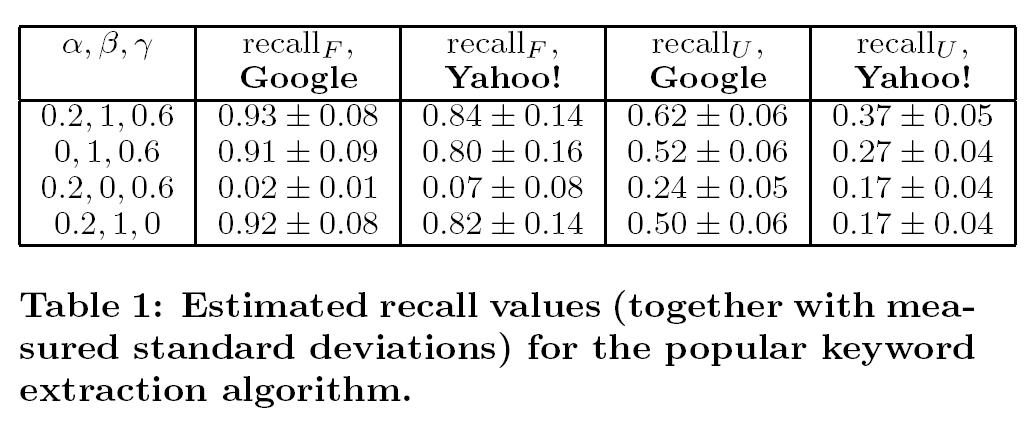
\includegraphics[width=100mm]{t1}
        \end{figure}
    \end{frame}

    \begin{frame}[plain]{Recall}
        \begin{figure}
        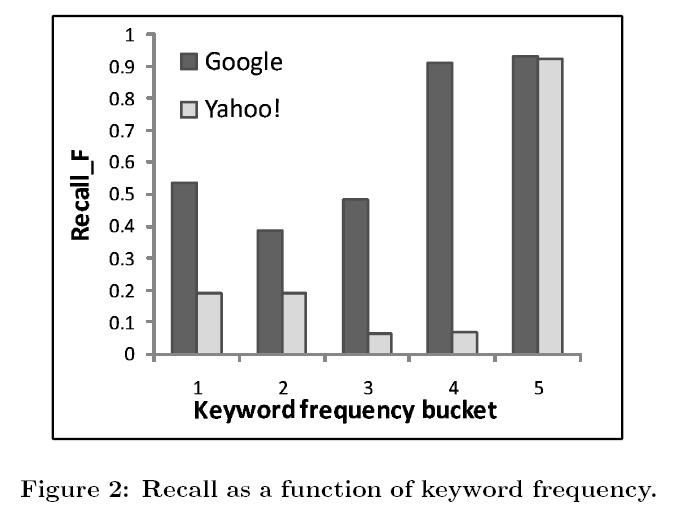
\includegraphics[width=100mm]{f2}
        \end{figure}
    \end{frame}

    \begin{frame}[plain]{Progress}
        \begin{figure}
        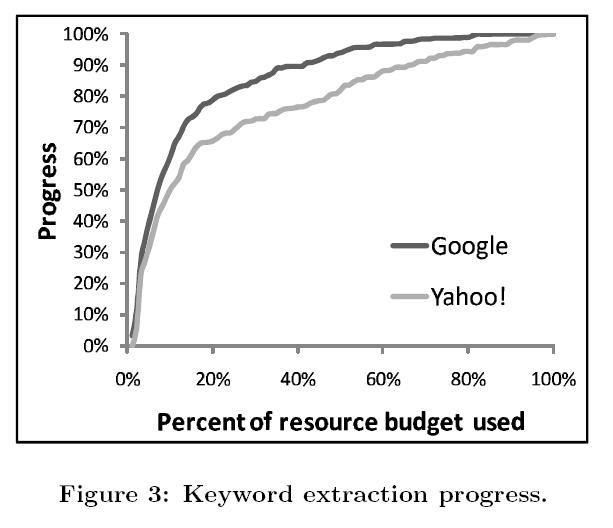
\includegraphics[width=100mm]{f3}
        \end{figure}
    \end{frame}

    \begin{frame}[plain]{ImpressionRank Estimates For News Sites}
        \begin{figure}
        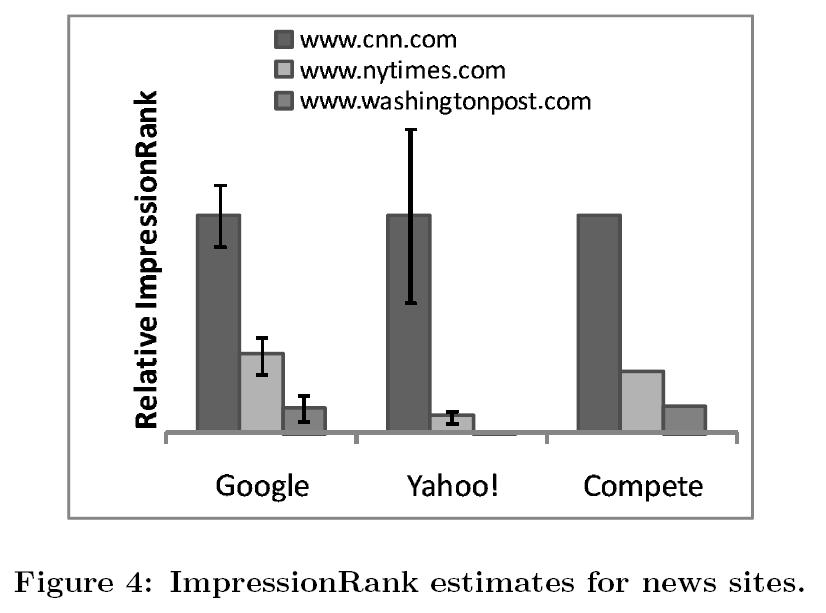
\includegraphics[width=100mm]{f4}
        \end{figure}
    \end{frame}

    \begin{frame}[plain]{ImpressionRank Estimates For Travel Sites}
        \begin{figure}
        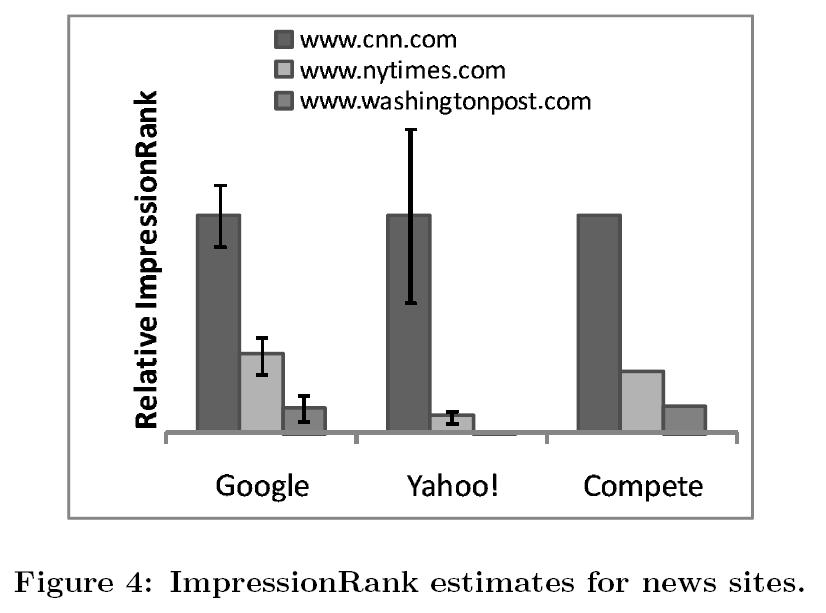
\includegraphics[width=100mm]{f4}
        \end{figure}
    \end{frame}

    \begin{frame}[plain]{Pupular Keywords}
        \begin{figure}
        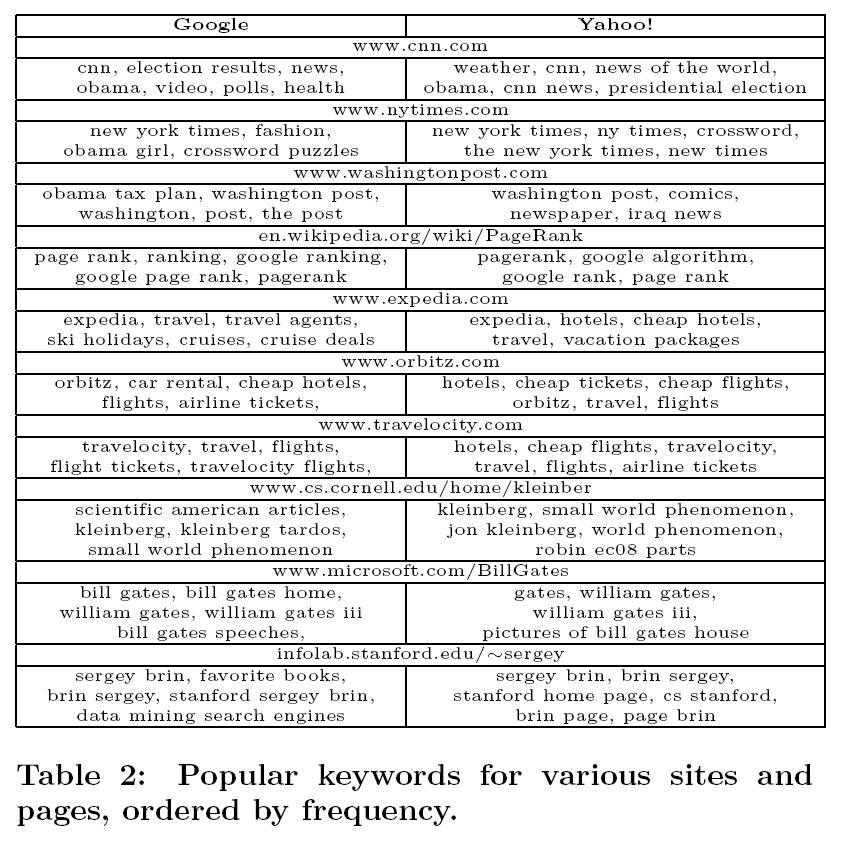
\includegraphics[width=100mm]{t2}
        \end{figure}
    \end{frame}

    \begin{frame}{Think Boldly!}
        \begin{center}
        \huge{Thanks ~}
        \end{center}
    \end{frame}

\end{document}


